\subsection{機能一覧}

本システムが提供する主要な機能は以下の通りである。

\subsubsection{EE-indexのプロット機能}
本システムの中核となる機能として、ブラウザ上でのEE-indexの時系列データの可視化が挙げられる。
ユーザーは任意の期間（1日、数日、1ヶ月など）および観測点を指定することで、対象となるEE-indexの変動をグラフとして確認することができる。
グラフはインタラクティブな操作に対応しており、拡大・縮小やカーソルホバーによる詳細な値の確認が可能である。
これにより、研究者はデータの全体的な傾向から微細な変動までをシームレスに分析することが可能となっている（図\ref{fig:web_ee-index_plot}）。

\begin{figure}[H]
  \centering
  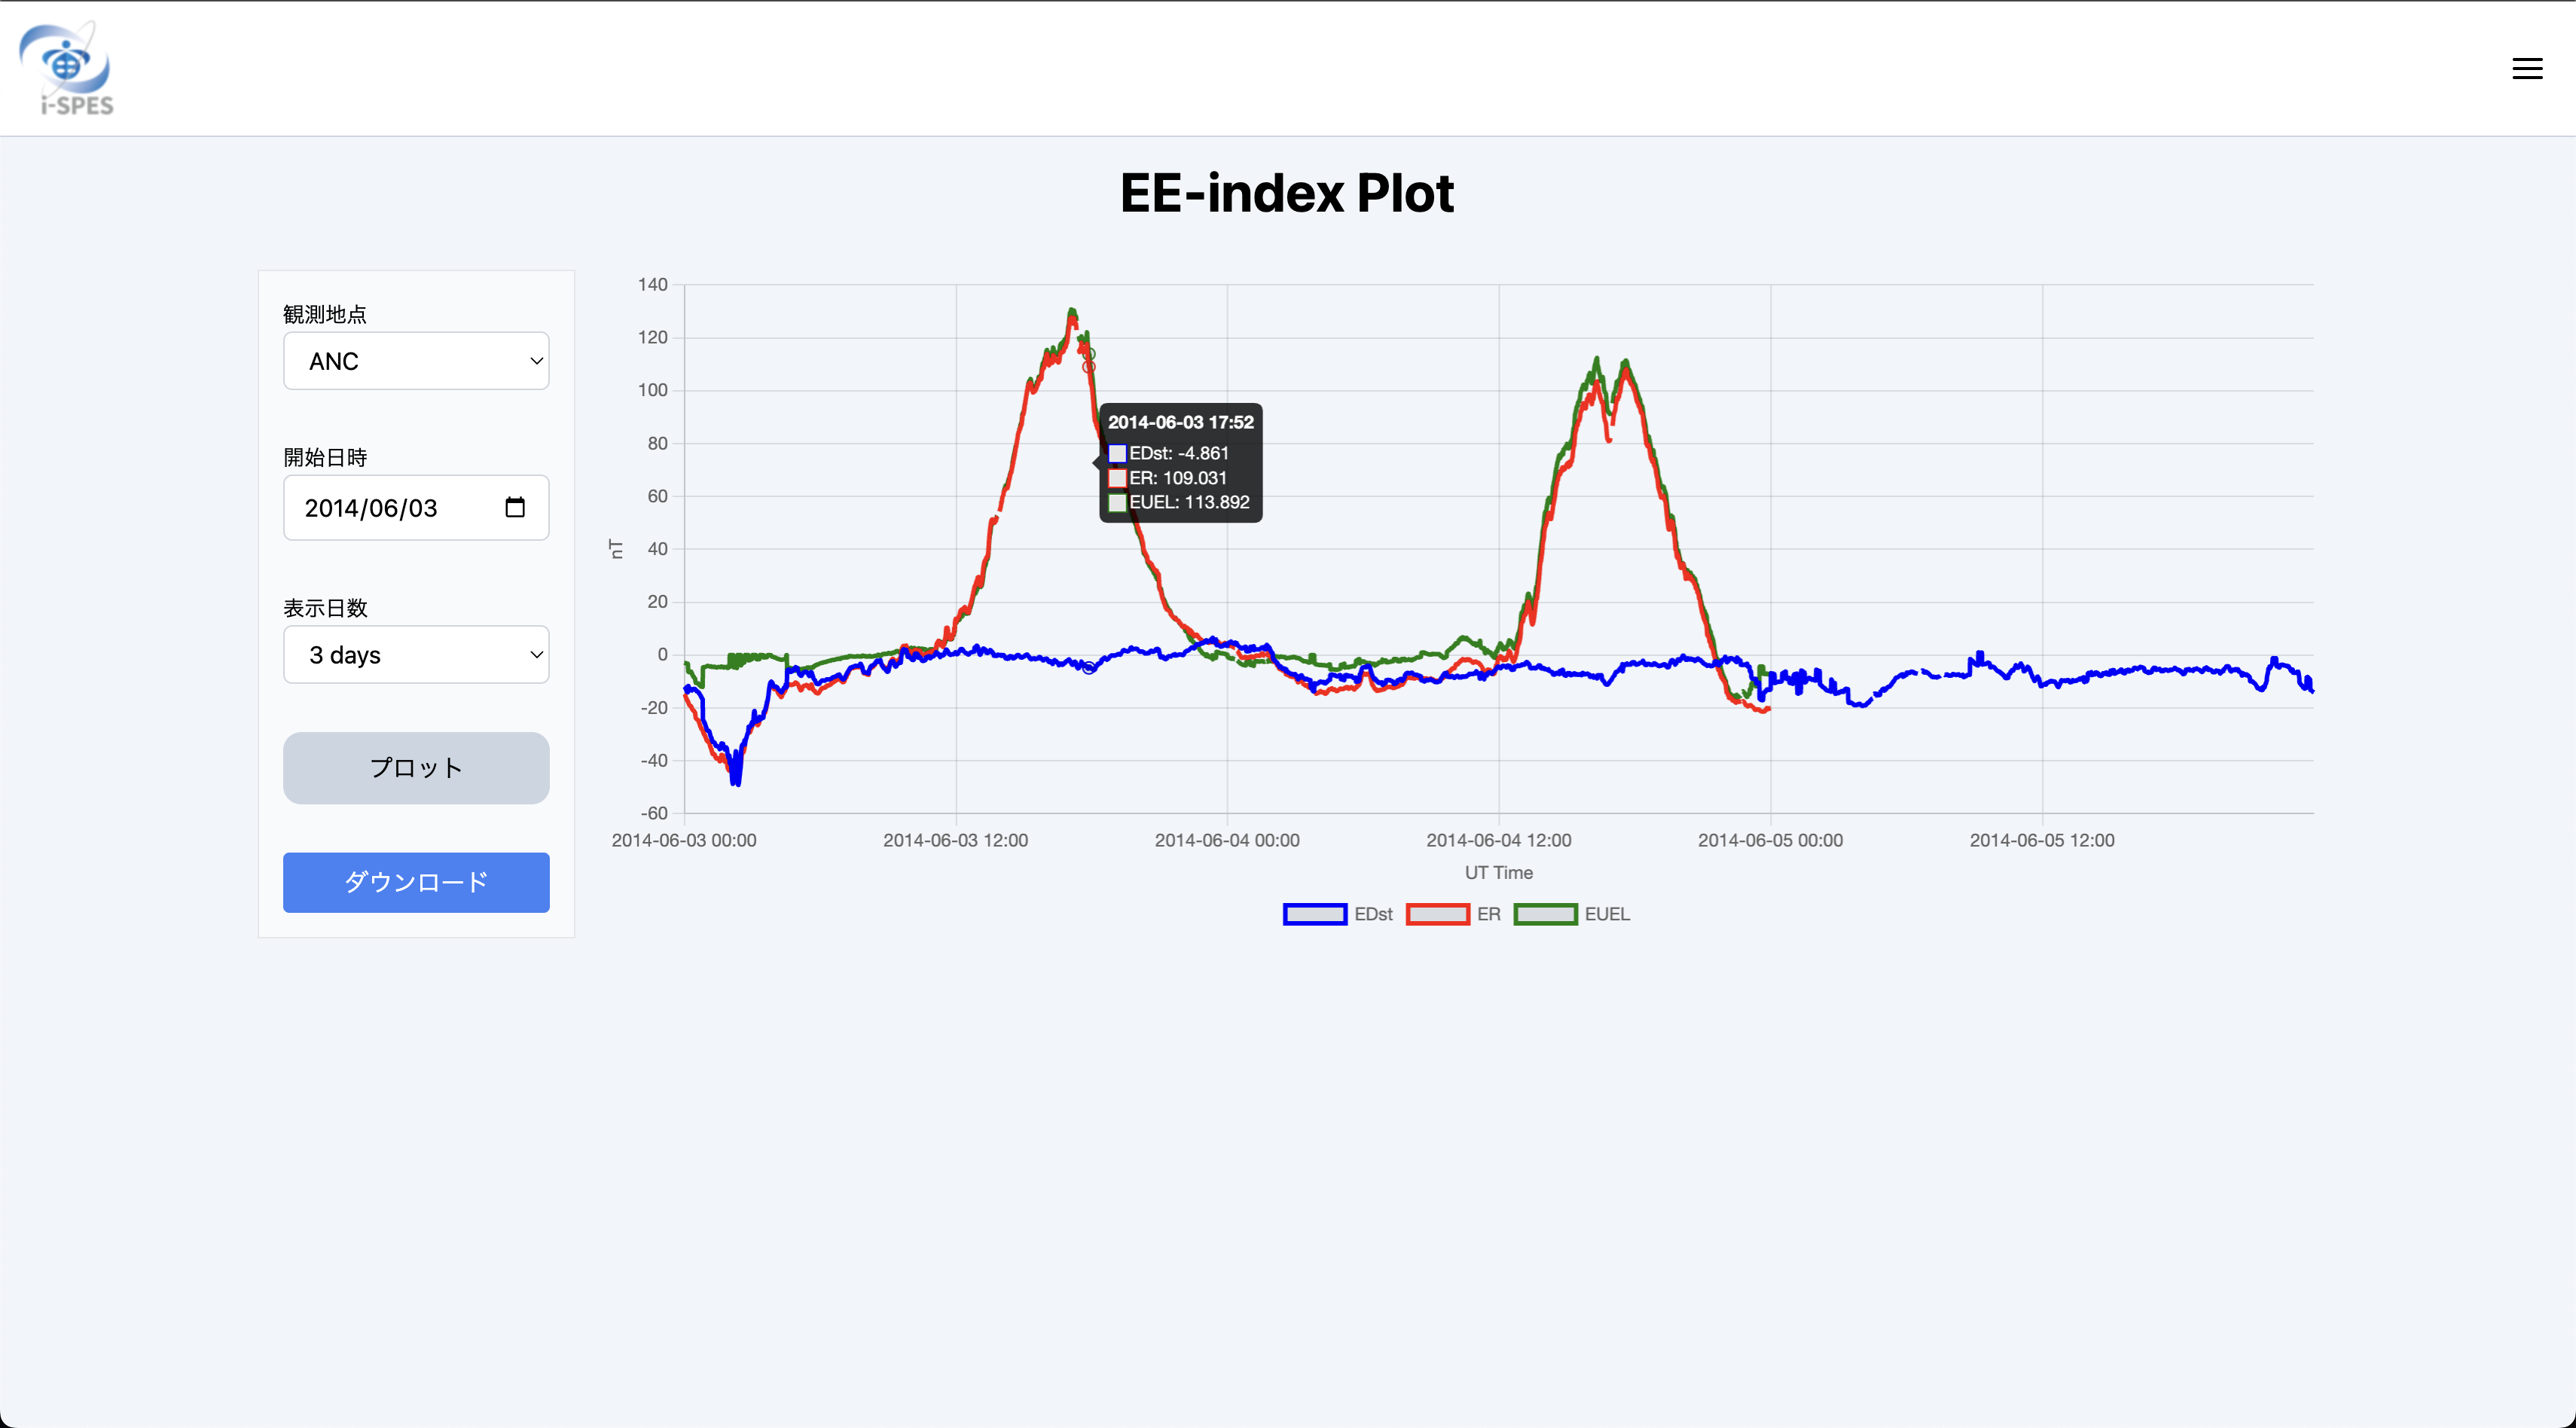
\includegraphics[width=\textwidth]{figures/web_ee-index_plot.png}
  \caption{EE-indexの時系列表示画面}
  \label{fig:web_ee-index_plot}
\end{figure}

\subsubsection{ローカルタイムのEUELのプロット機能}
EE-indexのプロット機能と同様に、ローカルタイムのEUELをプロットする機能であり、
任意の期間でのローカルの地磁気擾乱を捉えることが可能である。
また、前章で述べた特異型EEJ（Equatorial Electrojet）現象を自動的に検知する機能を活用して、
特異型EEJのイベントが存在する場合は、グラフ上でその日付が視覚的に強調表示される。
これにより、リアルタイムでローカルの地磁気擾乱が特異かどうかを瞬時に知ることが可能になる（図\ref{fig:web_euel_plot}）。

\begin{figure}[H]
  \centering
  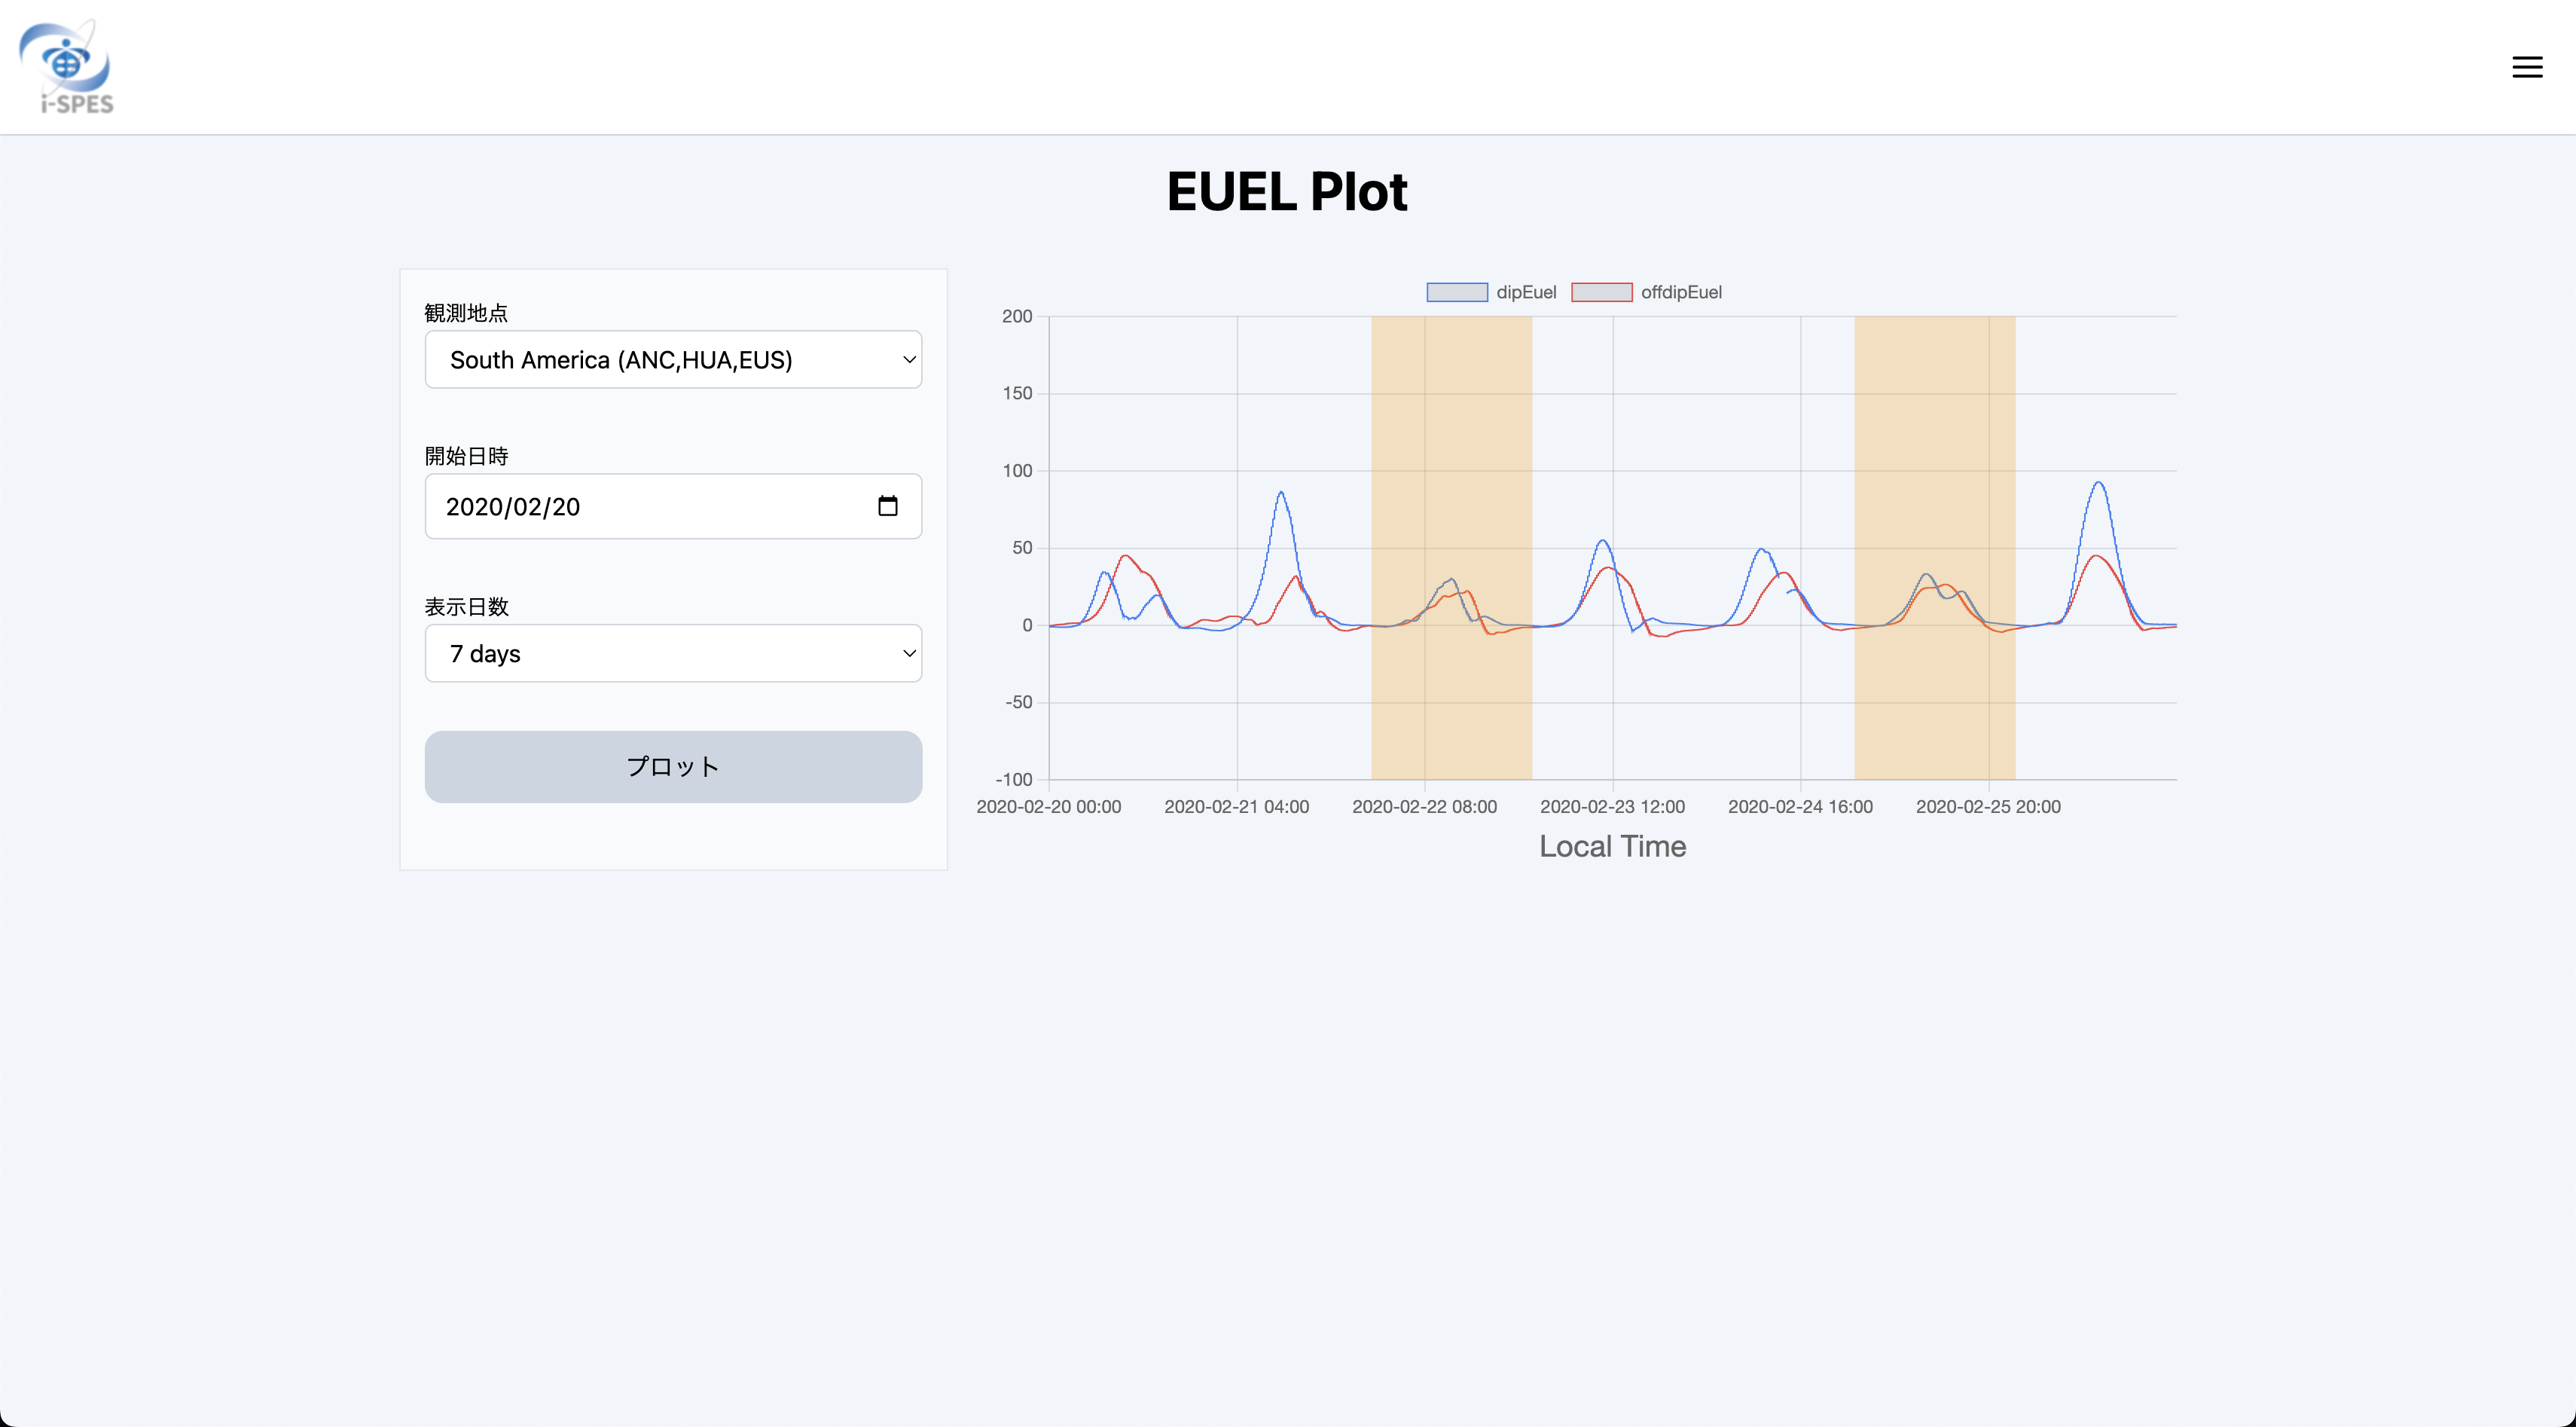
\includegraphics[width=\textwidth]{figures/web_euel_plot.png}
  \caption{特異型EEJ検知画面(色が塗られている日が特異型EEJが発生した日)}
  \label{fig:web_euel_plot}
\end{figure}

\subsubsection{MAGDAS観測データのダウンロード}
解析に使用されたEE-indexデータは、MAGDASプロジェクトで標準的に使用されているIAGA-2002フォーマットに準拠したテキストファイル（.iaga形式）としてダウンロード可能である。
また、複数日または長期間のデータを指定した場合には、それらをZIPファイルとして圧縮し、一括でダウンロードする機能も提供している。
これにより、ユーザーは取得したデータを手元のローカル環境で詳細に解析することが可能になる（図\ref{fig:web_ee-index_download}）。

\begin{figure}[H]
  \centering
  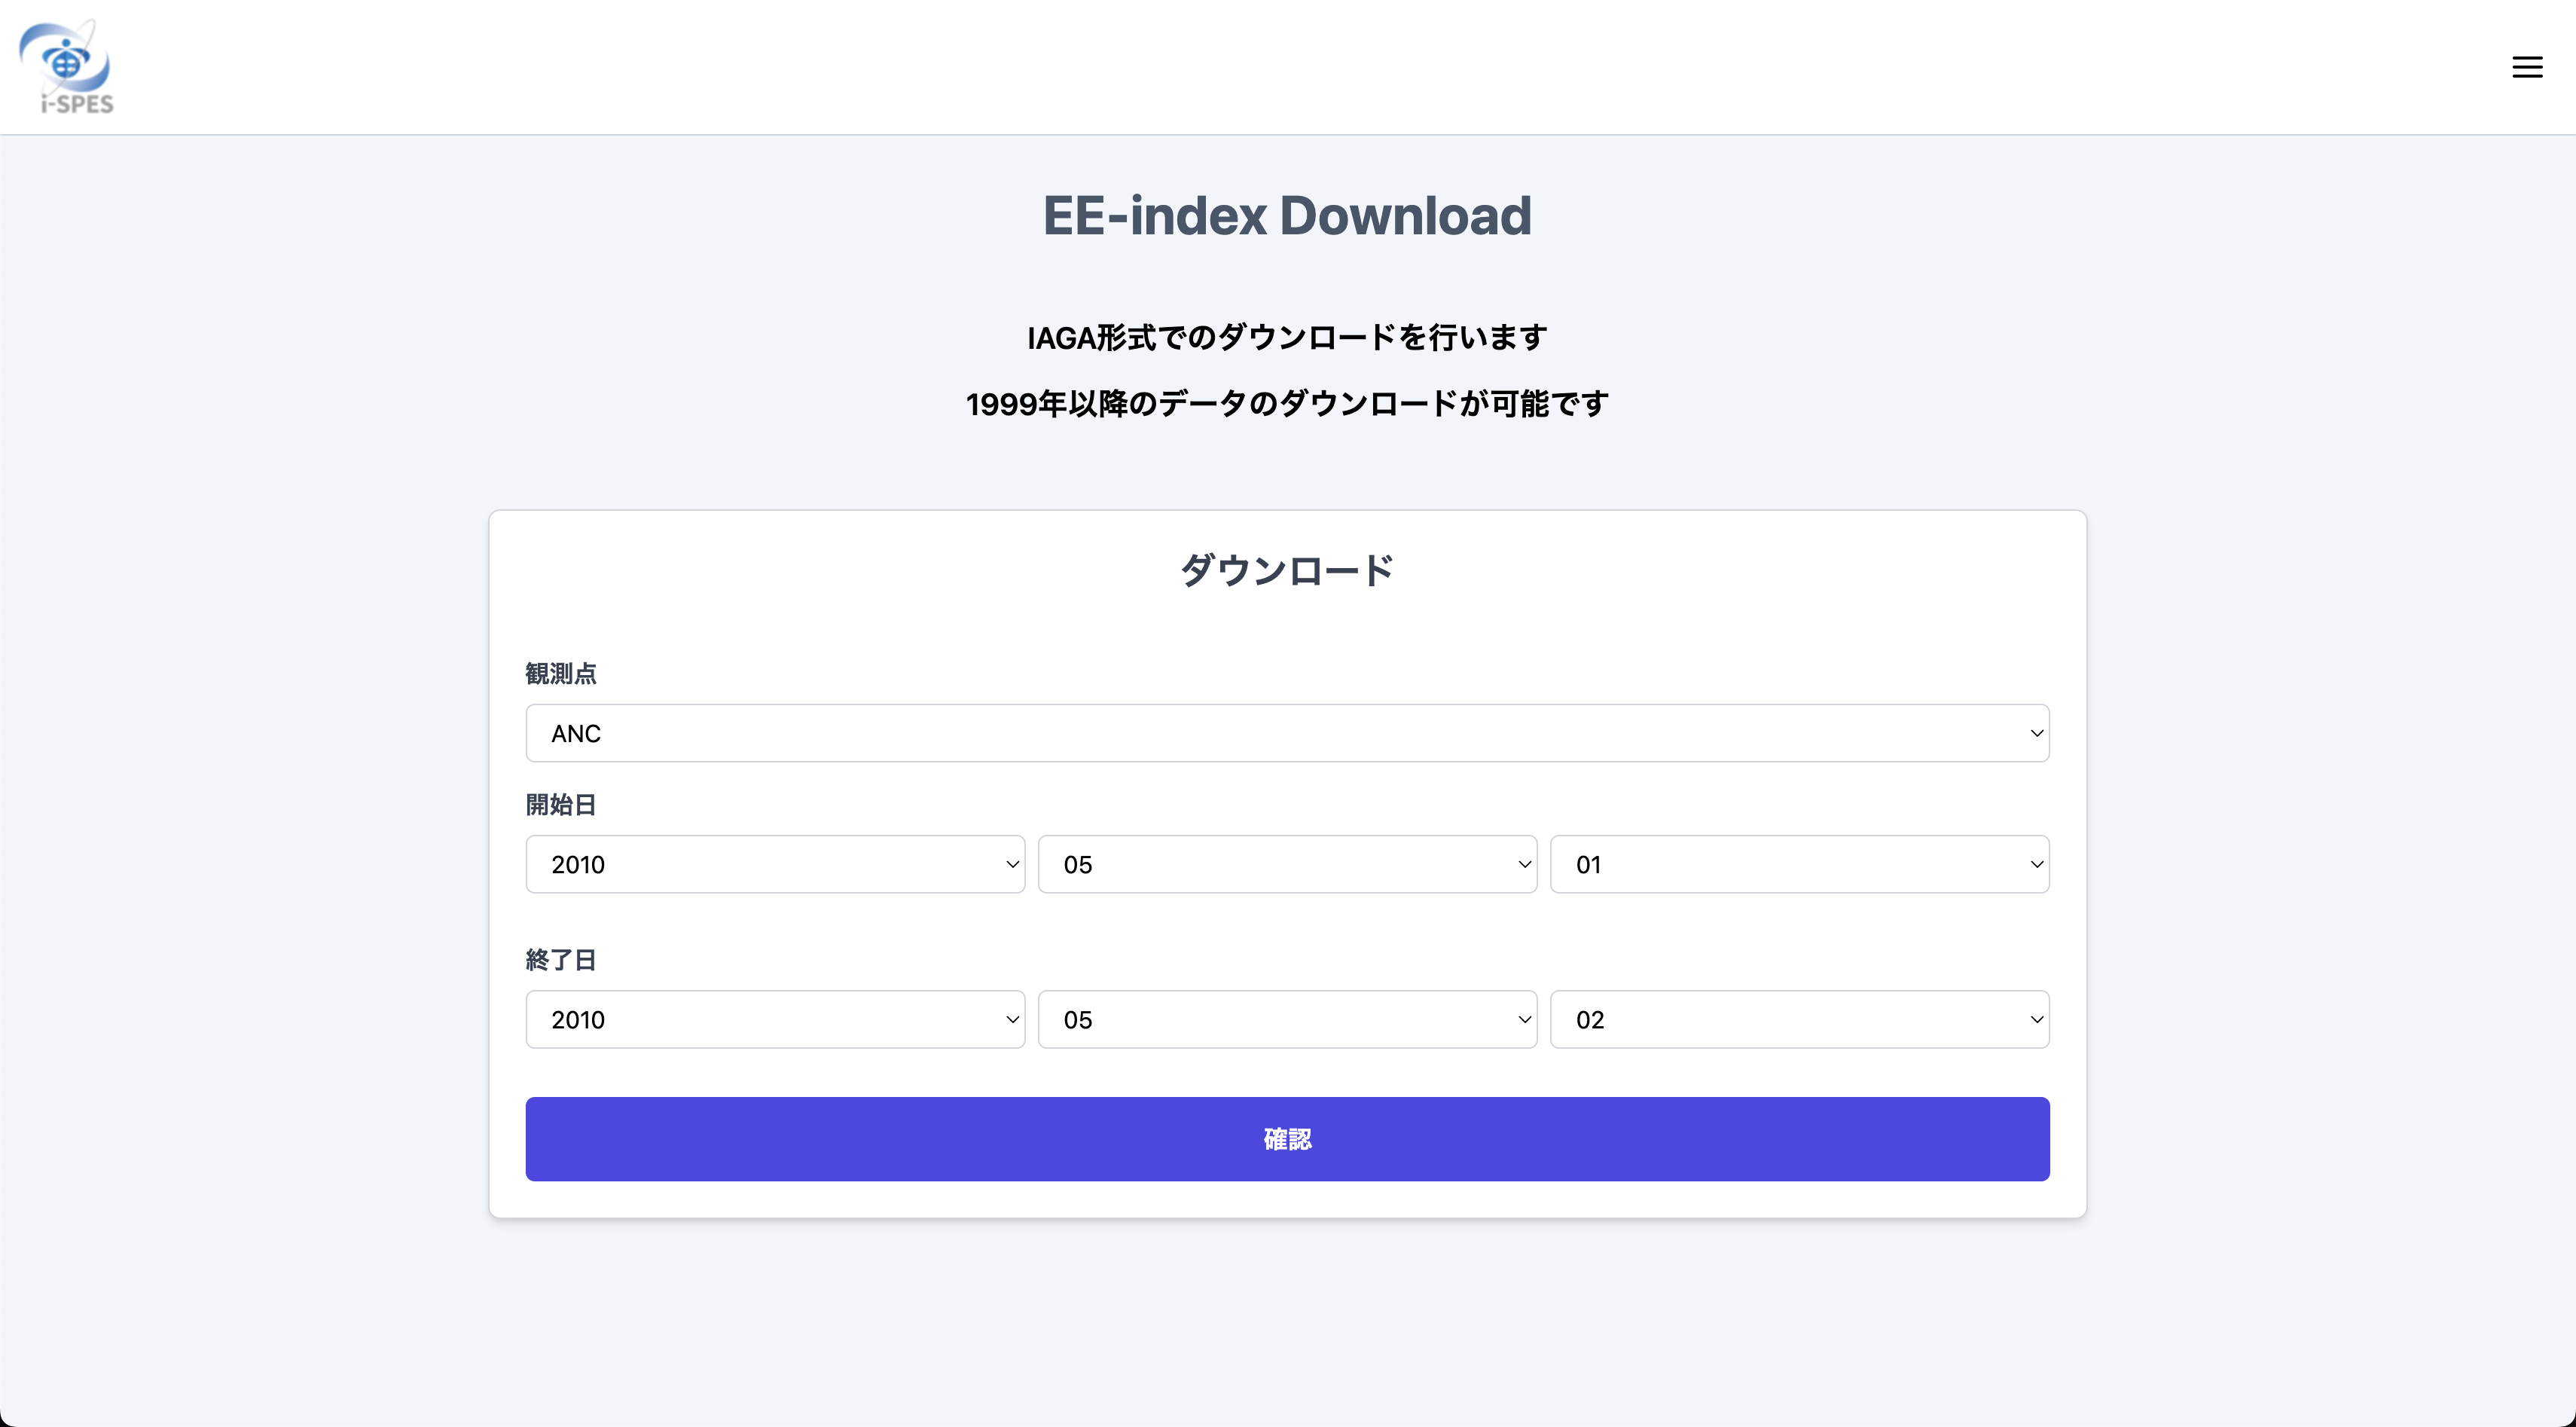
\includegraphics[width=0.8\textwidth]{figures/web_ee-index_download.png}
  \caption{MAGDAS観測データダウンロード画面}
  \label{fig:web_ee-index_download}
\end{figure}